\chapter {RESULTS}

\section{File System view after mounting}
The KWEST file system needs to be mounted by running a program and specifying a mount point. Once mounted, the file system can be used through any tool or application.
\subsection{Terminal View}
\begin{figure}[htb]
\centering
\setlength\fboxsep{0pt}
\setlength\fboxrule{0.5pt}
\fbox{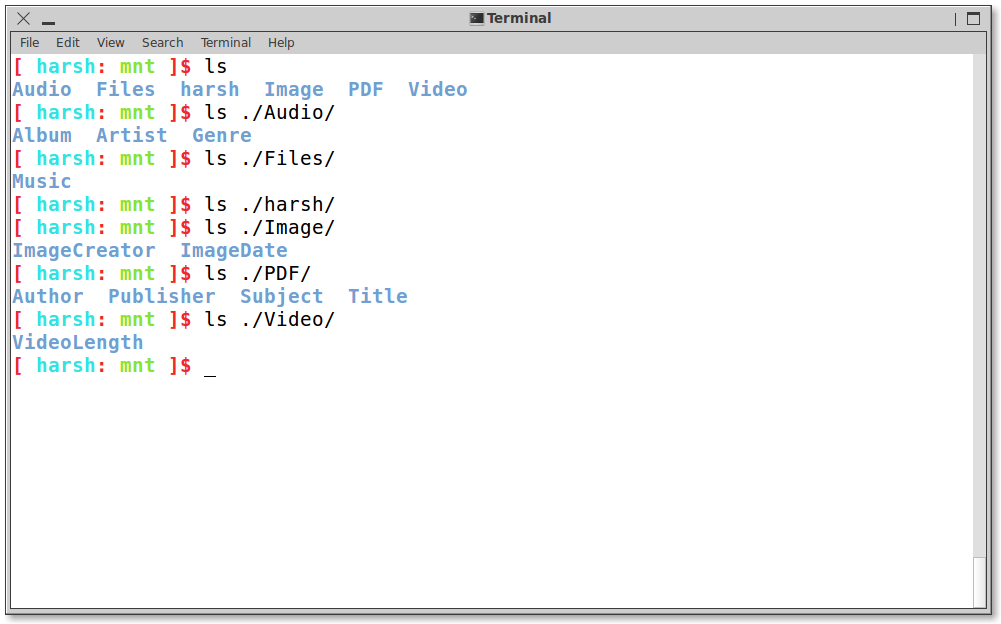
\includegraphics[width=0.8\linewidth]{./opimg/term_ls.png}}
%\includegraphics[width=0.8\textwidth]{image.png}
\caption{KWEST file systerm in Terminal after mounting}
\label{fig:dfd0}
\end{figure}

\subsection{File manager View}
A file manager or file browser is a computer program that provides a user interface to work with file systems. Files are typically displayed in a hierarchy. This is the default and only way traditional file systems can work. For semantic file systems like KWEST, virtual entries act like folders and files. These allow the file system to specify what entries to display without adhering to any strict hierarchy.

File managers used and tested with KWEST include: 
\begin{itemize}
\item Nautilus - The default file manager on Gnome distributions.
\item Nemo - The default file manager for Cinnamon desktop.
\item PCManFM - Lightweight file manager found in LXDE.
\item XFE - File manager for the X Window system.
\item Dolphin - The default file manager for KDE distributions.
\item Thunar - Fast and extendable file manager which supports plugins.
\end{itemize}

\begin{figure}[htb]
\centering
\setlength\fboxsep{0pt}
\setlength\fboxrule{0.5pt}
\fbox{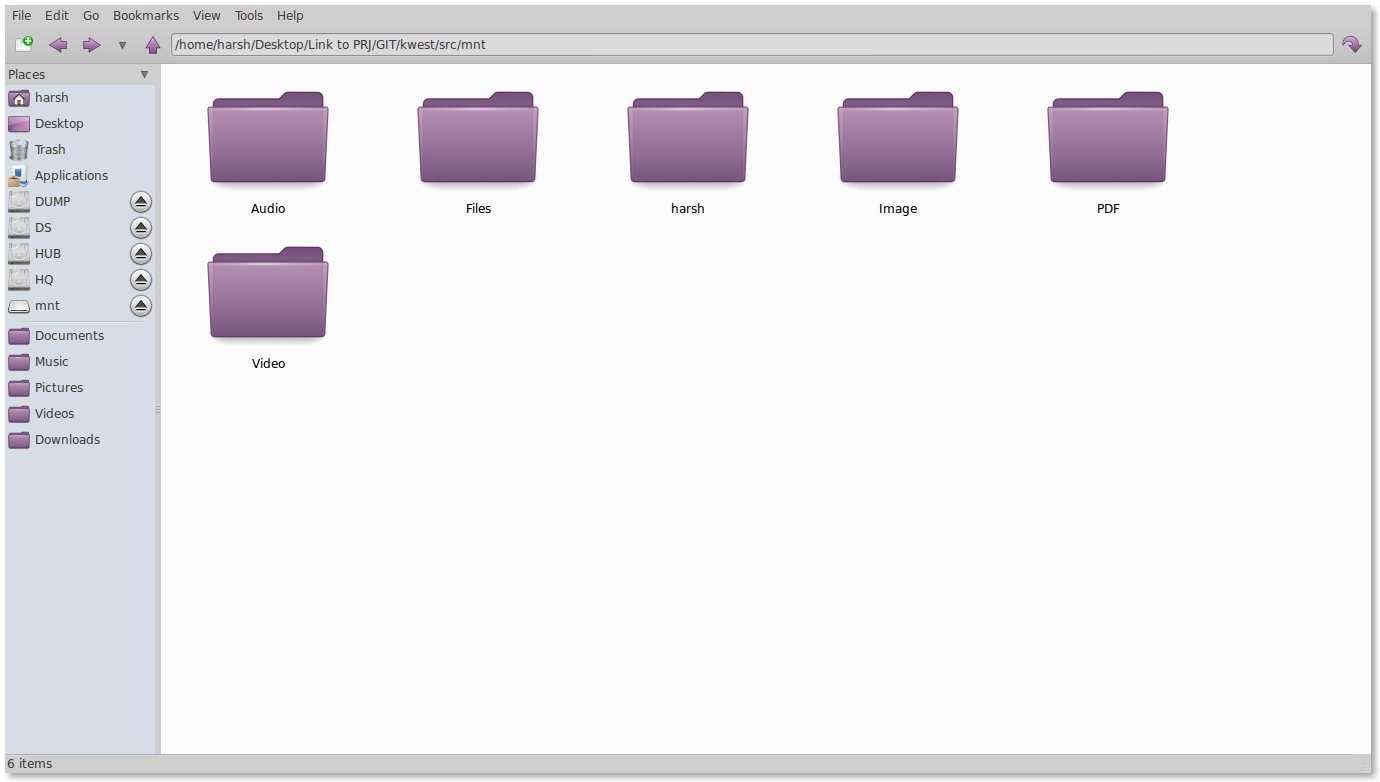
\includegraphics[width=0.8\linewidth]{./opimg/pcm_base.png}}
%\includegraphics[width=0.8\textwidth]{image.png}
\caption{KWEST file system in PCManFM after mounting}
\label{fig:dfd0}
\end{figure}
\newpage
\subsection{Organisation by File Types}
The KWEST file system extracts metadata from files while it is being imported. Depending on the extracted metadata, files are categorisedand put into folders corresponding to their types. Currently, KWEST supports the following file types:
\begin{enumerate}
\item Audio files
\item Images
\item PDF Documents
\item Videos
\end{enumerate}
The seperation of files into individual folders based on their types makes it easy to find a particular file. This is because each file type has its own metadata, which is used to categorise that file. An automated and organised view of files helps avoid clutter and provides efficient searching facilities.
\begin{figure}[htb]
\centering
\setlength\fboxsep{0pt}
\setlength\fboxrule{0.5pt}
\fbox{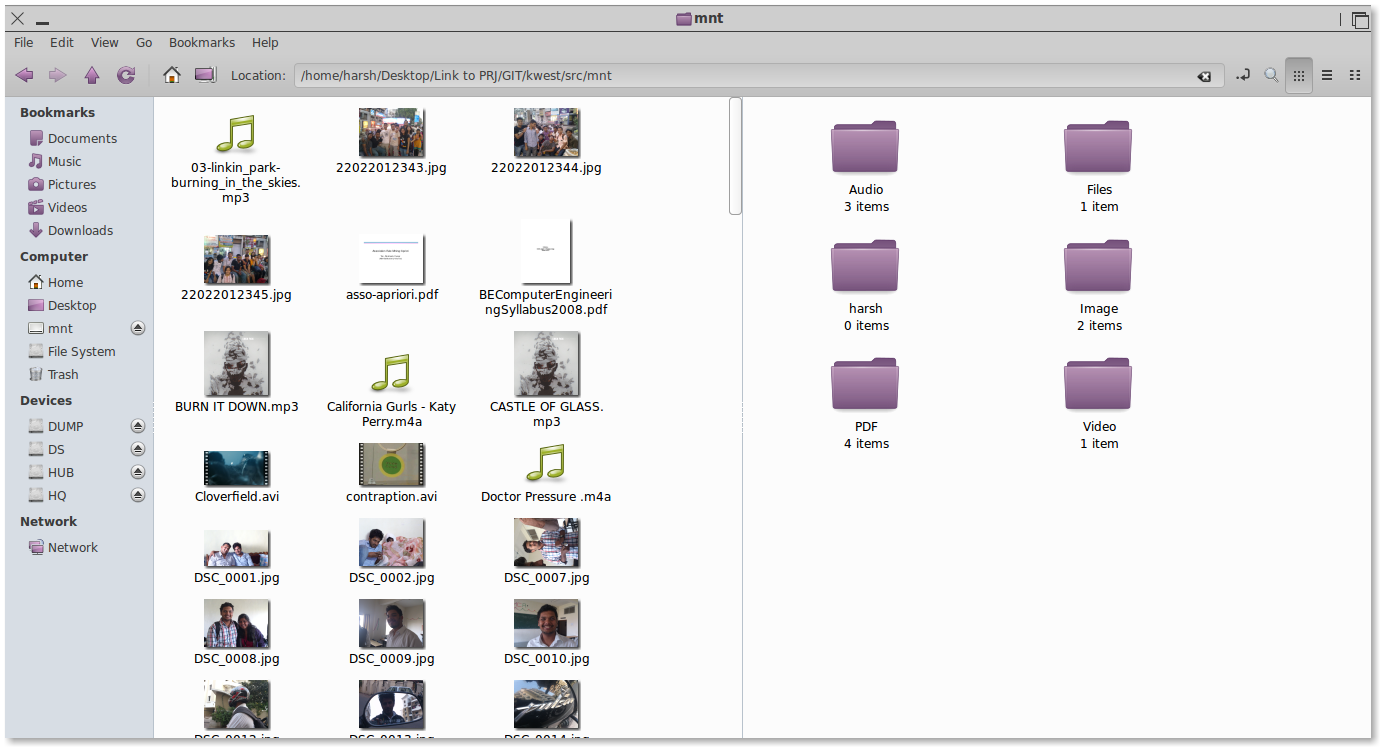
\includegraphics[width=0.8\linewidth]{./opimg/nemo_compare.png}}
%\includegraphics[width=0.8\textwidth]{image.png}
\caption{Chaotic organisation in normal file system vs KWEST auto-organisation}
\label{fig:dfd0}
\end{figure}

\section{Usage and Performance}
\begin{figure}[htb]
\centering
\setlength\fboxsep{0pt}
\setlength\fboxrule{0.5pt}
\fbox{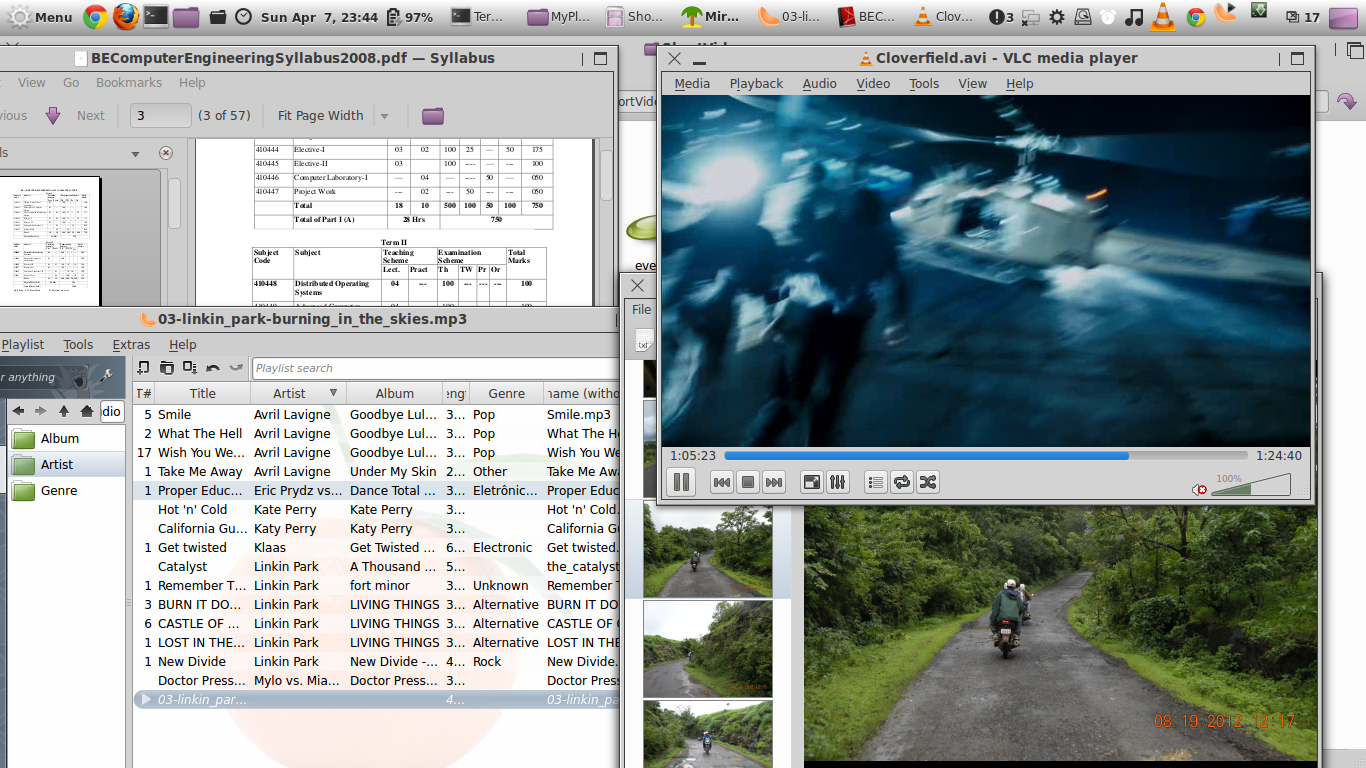
\includegraphics[width=0.8\linewidth]{./opimg/kwestusage.png}}
%\includegraphics[width=0.8\textwidth]{image.png}
\caption{Performance test for KWEST with normal user task loads}
\label{fig:dfd0}
\end{figure}
Although KWEST is a virtual file system, it can be used for normal daily tasks such as listening to music, reading documents, watching videos, etc. In the screenshot below, the applications each run or open a file on the KWEST file system simultaneously. No perceptible lag or performance degradation was noticed while playing music or watching the video. The file system performed sufficiently well in all four application operations.

\section{Suggestions}
Suggestions are files which are not actually present in that tag, but can be tagged as per the system's recommendation. There are two types of suggestions:
\begin{itemize}
\item \textbf{Probably Related} : The files probably belong to the tag, but the system is not sure about it.
\item \textbf{Related} : The file definately belogns to the tag, and the user can tag it.
\end{itemize}
\begin{figure}[htb]
\centering
\setlength\fboxsep{0pt}
\setlength\fboxrule{0.5pt}
\fbox{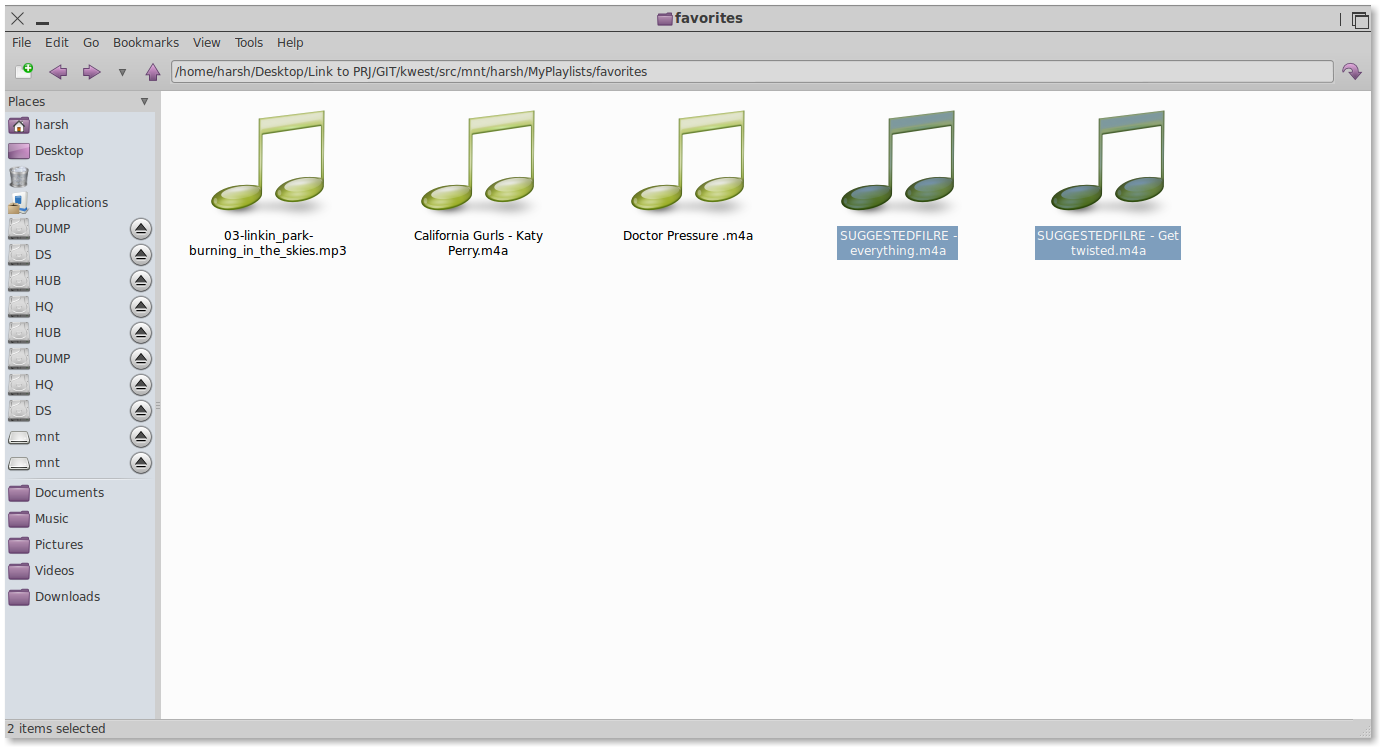
\includegraphics[width=0.8\linewidth]{./opimg/suggestions.png}}
%\includegraphics[width=0.8\textwidth]{image.png}
\caption{KWEST showing suggestions for including files in the favorites tag}
\label{fig:dfd0}
\end{figure}

\section{Exporting files}
\begin{figure}[htb]
\centering
\setlength\fboxsep{0pt}
\setlength\fboxrule{0.5pt}
\fbox{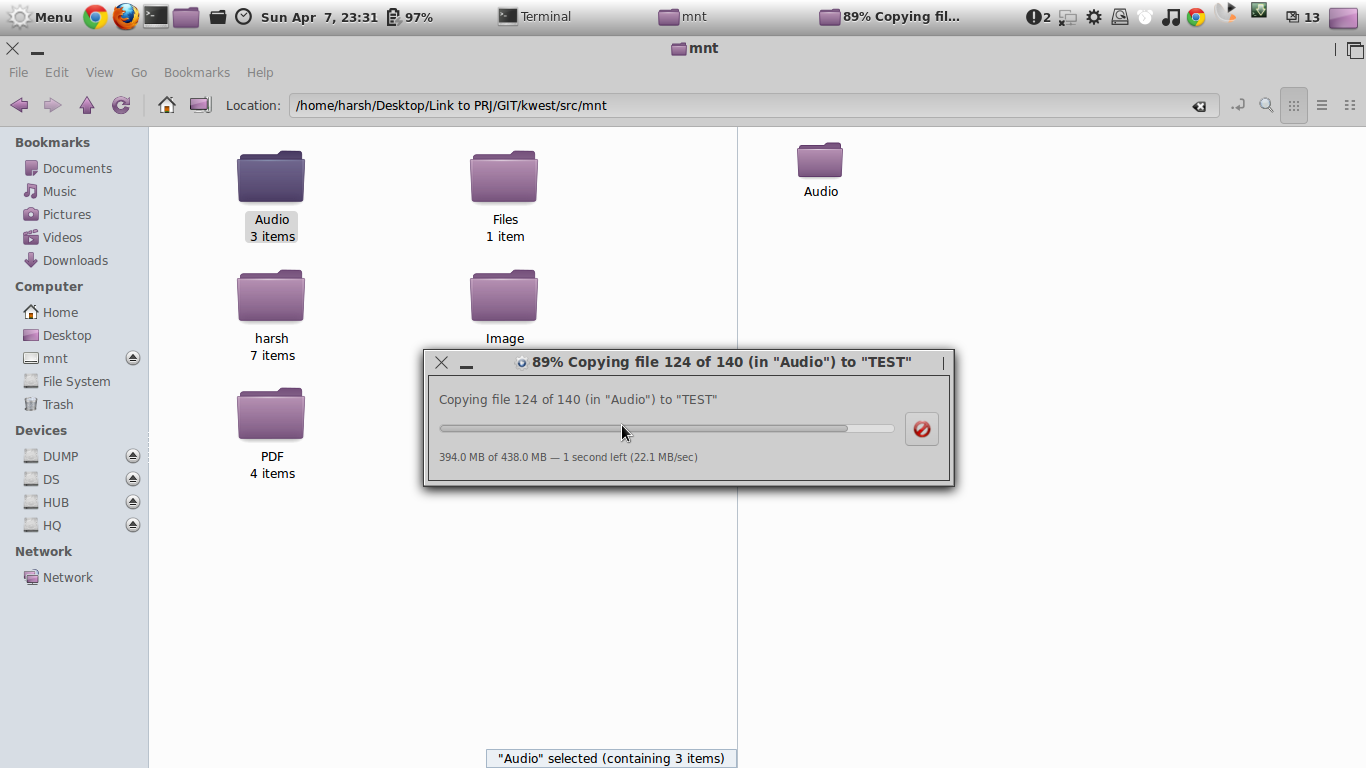
\includegraphics[width=0.8\linewidth]{./opimg/export2.png}}
%\includegraphics[width=0.8\textwidth]{image.png}
\caption{KWEST Export function - Copy file to external location}
\label{fig:dfd0}
\end{figure}
The entries, files, tags in KWEST are all virtual entries. They do not exist anywhere on a physical disk. In order to ``export'' this organisation to another location outside of KWEST, there is the \emph{Export} feature. Practically there is not difference between a normal copy and export. Export copies the virtual entries as real files by physically accessing the location where they are stored, and then copying them. To the end user, there is no increase in steps or time for the copying to complete.